\section{System Architecture}
        identificar componentes e suas ligacoes

        The project still follows the same System Structure that was established initially in the proposal, which has two major components and a 
        third exterior one, communicating with each other, separating concerns and business logic. The following figure illustrates the system's structure:
        
        The system architecture organizes the system's necessities into manageable blocks shown in figure TODO FIGURE LINK.
        It is essentially divided into two major components, the Client Application and the Service.
        
        The role of the Client Application is to provide an interface which the user can interact with. This component communicates 
        with either the Social Routing Service or external services when required. This communication is done through the HTTP protocol.
        
        The Social Routing Service processes and stores data that the Client Application can use at any time, as long as the authentication
        is correct.  

        \begin{figure}[h]            
            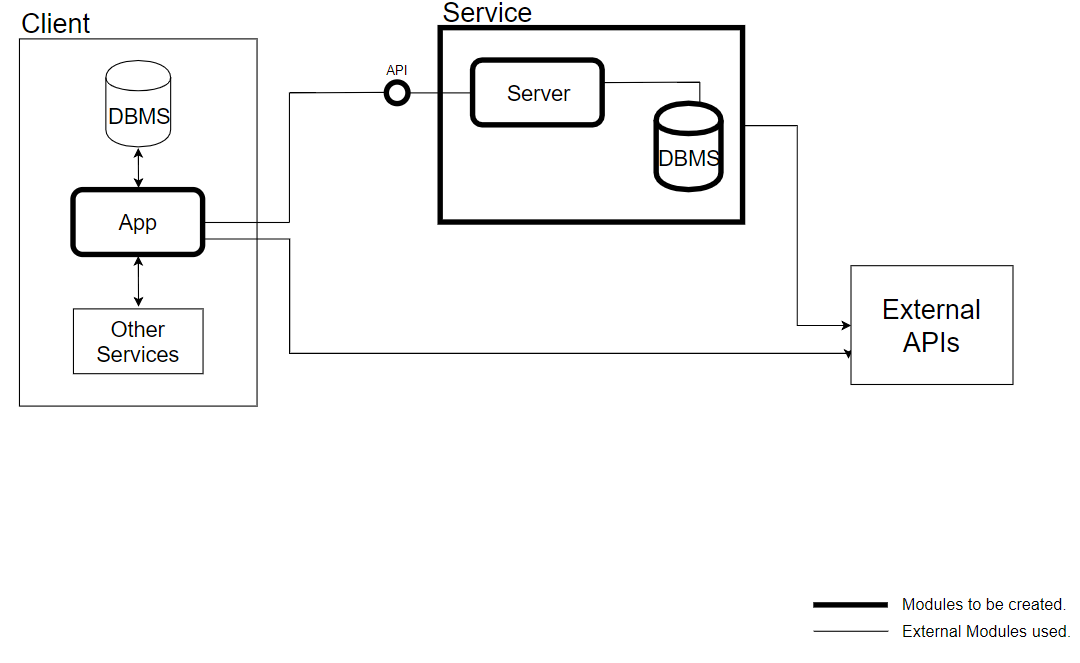
\includegraphics[width=\textwidth]{images/project-structure/system-structure.PNG}
            \caption{System structure.}
            \label{fig:systemstructure}
        \end{figure}  